\documentclass{beamer}
\usetheme{Madrid}

\usepackage{amsmath, amssymb, amsthm}
\usepackage{graphicx}
\usepackage{listings}
\usepackage[utf8]{inputenc}
\usepackage{hyperref}

\title{9.1.5}
\author{EE24BTECH11030 - Kedarananda}
\date{}

\begin{document}

\frame{\titlepage}

\begin{frame}
\frametitle{Question}
Solve the differential equation:
\begin{align*}
    \frac{d^2y}{dx^2} + 5x \left( \frac{dy}{dx} \right)^2 - 6y = \ln(x)
\end{align*}
\end{frame}

\begin{frame}
\frametitle{Solution: Theoretical Approach}
Given:
\begin{align}
    \frac{d^2y}{dx^2} + 5x \left( \frac{dy}{dx} \right)^2 - 6y &= \ln(x)
\end{align}
\newline
Since the equation is nonlinear, direct analytical solutions are challenging. Computational approaches such as \textbf{Euler's Method} or higher-order methods are used for approximations.
\end{frame}

\begin{frame}
\frametitle{Solution: Computational Approach}
The given equation is reformulated as:
\begin{align}
    y_1 &= y, \quad y_2 = \frac{dy}{dx} \\
    \frac{dy_1}{dx} &= y_2 \\
    \frac{dy_2}{dx} &= \ln(x) - 5x(y_2)^2 + 6y_1
\end{align}
The system of equations is solved iteratively using numerical techniques.
\newline
\textbf{Initial Conditions:}
\begin{itemize}
    \item $y(0.01) = 0.01$
    \item $y'(0.01) = 1$
    \item Step size $h = 0.01$
\end{itemize}
\end{frame}

\begin{frame}
\frametitle{Numerical Method: Euler's Method}
Using Euler's method:
\begin{align}
    \myvec{y_{1, n+1} \\ y_{2, n+1}} = \myvec{y_{1, n} \\ y_{2, n}} 
    + h \cdot \myvec{y_{2, n} \\ \ln(x_n) - 5x_n (y_{2, n})^2 + 6y_{1, n}}
\end{align}
This update is applied iteratively for all $x_n$ values to compute $y(x)$ and $y'(x)$.
\end{frame}

\begin{frame}
\frametitle{Comparison of Results}
\begin{figure}[h!]
    \centering
    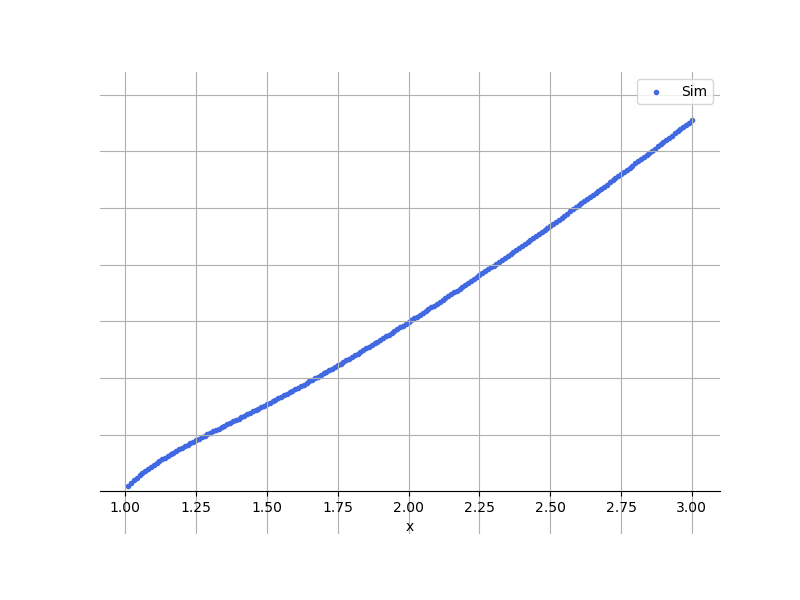
\includegraphics[width=\columnwidth]{figs/fig1.png} % Replace with the generated plot file
    \caption{Comparison of $y(x)$: Theoretical vs Computational}
    \label{comparison}
\end{figure}
\end{frame}

\begin{frame}{allowframebreaks}
\frametitle{C-Code}
\begin{figure}[ht]
    \centering
    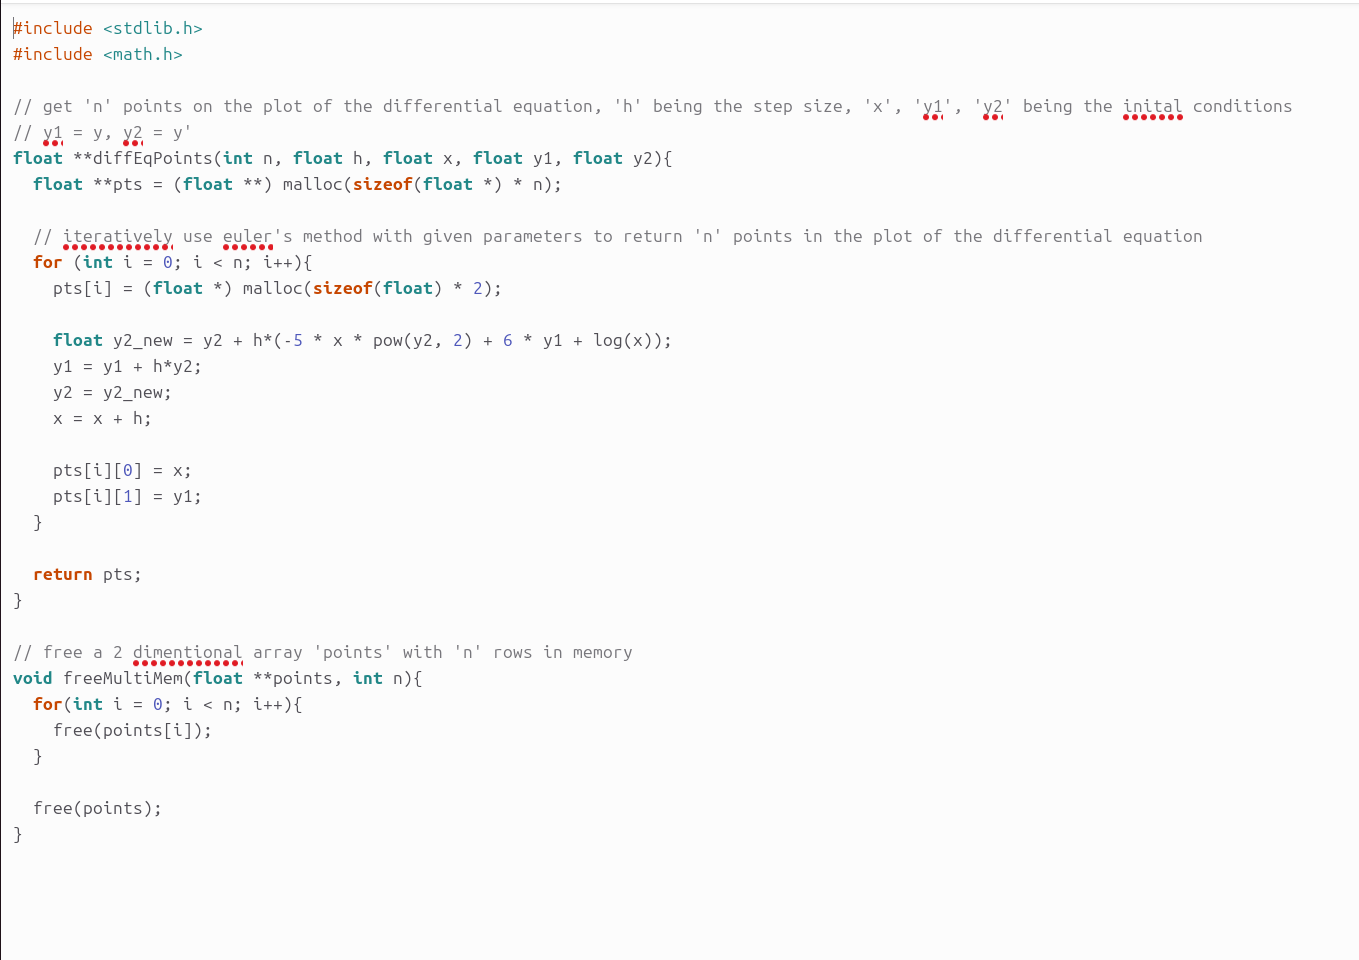
\includegraphics[width=\columnwidth]{fig2.png} % Replace with your C code snippet
\end{figure}
\end{frame}

\begin{frame}{allowframebreaks}
\frametitle{Code for Plot}
\begin{figure}[ht]
    \centering
    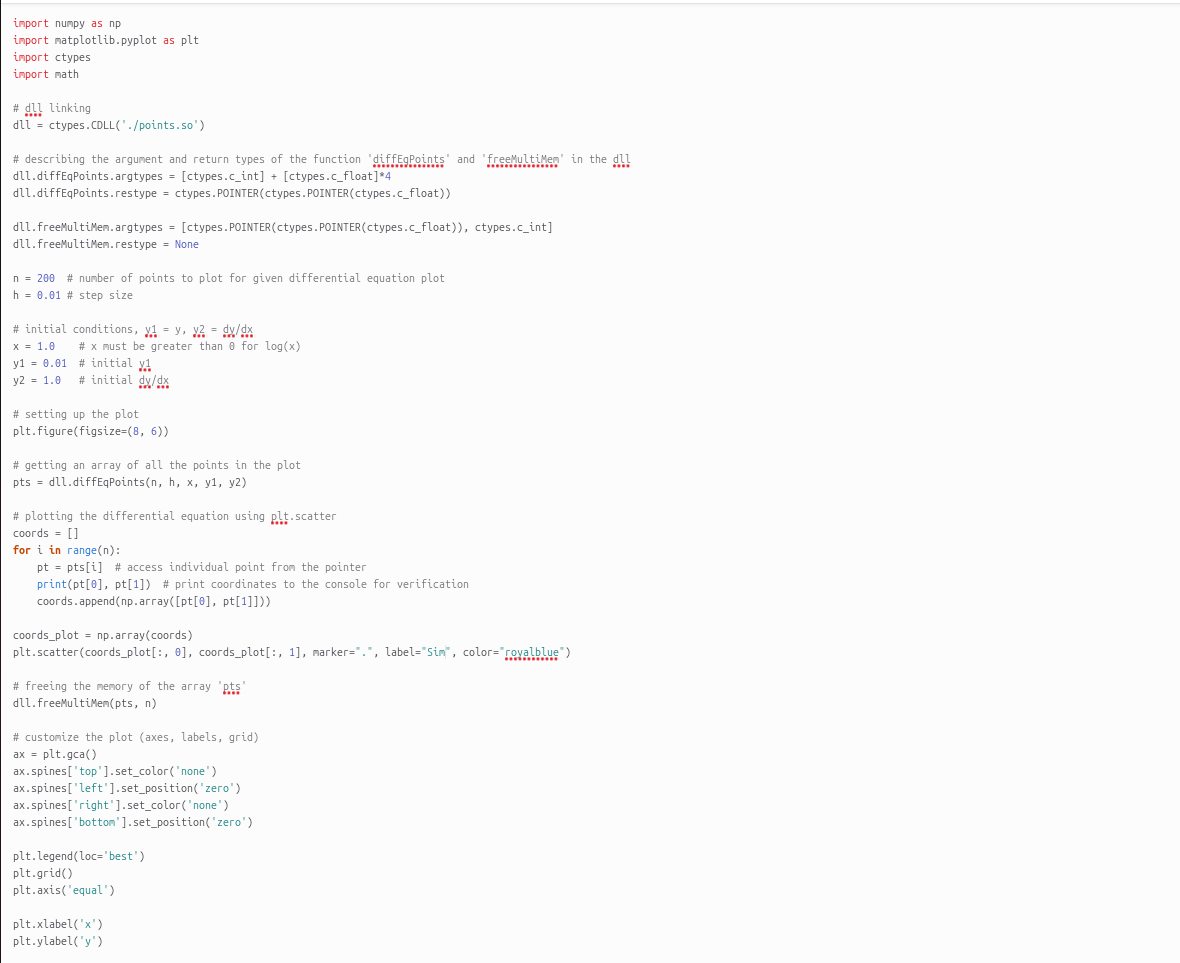
\includegraphics[width=6cm, height=8cm]{fig3.png} % Replace with the plotting code snippet
\end{figure}
\end{frame}

\end{document}

